% Choose one to switch between slides and handout
\documentclass[]{beamer}
%\documentclass[handout]{beamer}

% Video Meta Data
\title{Bitcoin, Blockchain and Cryptoassets}
\subtitle{Block Assembly \& Chain Structure}
\author{Prof. Dr. Fabian Schär}
\institute{University of Basel}

% Config File
% Packages
\usepackage[utf8]{inputenc}
\usepackage{hyperref}
\usepackage{gitinfo2}
\usepackage{tikz}
\usepackage{amsmath}
\usepackage{mathtools}
\usepackage{bibentry}
\usepackage{xcolor}
\usepackage{colortbl} % Add colour to LaTeX tables
\usepackage{caption}
\usepackage[export]{adjustbox}
\usepackage{pgfplots} \pgfplotsset{compat = 1.17}
\usepackage{makecell}
\usepackage{fancybox}
\usepackage{ragged2e}
\usepackage{fontawesome}
\usepackage{seqsplit}
\usepackage{tabularx}

% Color Options
\definecolor{highlight}{rgb}{0.65,0.84,0.82}
\definecolor{focus}{rgb}{0.72, 0, 0}
\definecolor{lightred}{rgb}{0.8,0.5,0.5}
\definecolor{midgray}{RGB}{190,195,200}

% Beamer Template Options
\beamertemplatenavigationsymbolsempty
\setbeamertemplate{footline}[frame number]
\setbeamercolor{structure}{fg=black}
\setbeamercolor{footline}{fg=black}
\setbeamercolor{title}{fg=black}
\setbeamercolor{frametitle}{fg=black}
\setbeamercolor{item}{fg=black}
\setbeamercolor{}{fg=black}
\setbeamercolor{bibliography item}{fg=black}
\setbeamercolor*{bibliography entry title}{fg=black}
\setbeamercolor{alerted text}{fg=focus}
\setbeamertemplate{items}[square]
\setbeamertemplate{enumerate items}[default]
\captionsetup[figure]{labelfont={color=black},font={color=black}}
\captionsetup[table]{labelfont={color=black},font={color=black}}

\setbeamertemplate{bibliography item}{\insertbiblabel}

% Link Icon Command
\newcommand{\link}{%
    \tikz[x=1.2ex, y=1.2ex, baseline=-0.05ex]{%
        \begin{scope}[x=1ex, y=1ex]
            \clip (-0.1,-0.1)
                --++ (-0, 1.2)
                --++ (0.6, 0)
                --++ (0, -0.6)
                --++ (0.6, 0)
                --++ (0, -1);
            \path[draw,
                line width = 0.5,
                rounded corners=0.5]
                (0,0) rectangle (1,1);
        \end{scope}
        \path[draw, line width = 0.5] (0.5, 0.5)
            -- (1, 1);
        \path[draw, line width = 0.5] (0.6, 1)
            -- (1, 1) -- (1, 0.6);
        }
    }

% Read Git Data from Github Actions Workflow
% Defaults to gitinfo2 for local builds
\IfFileExists{gitInfo.txt}
	{\input{gitInfo.txt}}
	{
		\newcommand{\gitRelease}{(Local Release)}
		\newcommand{\gitSHA}{\gitHash}
		\newcommand{\gitDate}{\gitAuthorIsoDate}
	}

% Custom Titlepage
\defbeamertemplate*{title page}{customized}[1][]
{
  \vspace{-0cm}\hfill\includegraphics[width=2.5cm]{../config/logo_cif}
  \includegraphics[width=1.9cm]{../config/seal_wwz}
  \\ \vspace{2em}
  \usebeamerfont{title}\textbf{\inserttitle}\par
  \usebeamerfont{title}\usebeamercolor[fg]{title}\insertsubtitle\par  \vspace{1.5em}
  \small\usebeamerfont{author}\insertauthor\par
  \usebeamerfont{author}\insertinstitute\par \vspace{2em}
  \usebeamercolor[fg]{titlegraphic}\inserttitlegraphic
    \tiny \noindent \texttt{Release Ver.: \gitRelease}\\ 
    \texttt{Version Hash: \gitSHA}\\
    \texttt{Version Date: \gitDate}\\ \vspace{1em}
    
    
    \iffalse
  \link \href{https://github.com/cifunibas/Bitcoin-Blockchain-Cryptoassets/blob/main/slides/intro.pdf}
  {Get most recent version}\\
  \link \href{https://github.com/cifunibas/Bitcoin-Blockchain-Cryptoassets/blob/main/slides/intro.pdf}
  {Watch video lecture}\\ 
  
  \fi
  
  \vspace{1em}
  License: \texttt{Creative Commons Attribution-NonCommercial-ShareAlike 4.0 International}\\\vspace{2em}
  \includegraphics[width = 1.2cm]{../config/license}
}


% tikzlibraries
\usetikzlibrary{decorations.pathreplacing}
\usetikzlibrary{decorations.markings}
\usetikzlibrary{positioning}
\usetikzlibrary{calc}
\captionsetup{font=footnotesize}


%%%%%%%%%%%%%%%%%%%%%%%%%%%%%%%%%%%%%%%%%%%%%%
%%%%%%%%%%%%%%%%%%%%%%%%%%%%%%%%%%%%%%%%%%%%%%
\begin{document}

\thispagestyle{empty}
\begin{frame}[noframenumbering]
	\titlepage
\end{frame}

%%%
\begin{frame}{Transaction Distribution}
\begin{figure}
	\centering
	\begin{tikzpicture}[scale=0.9, every node/.style={scale=0.9}]
		% Network
\node (agenta) at (1,2.8) {\includegraphics[width = 0.6 cm]{../assets/images/agents/avatar_rand3.png}};
\node (agentb) at (0.5,1) {\includegraphics[width = 0.6 cm]{../assets/images/agents/avatar_rand4.png}};
\node (agentc) at (3,2.1) {\includegraphics[width = 0.6 cm]{../assets/images/agents/avatar_rand5.png}};
\node (agente) at (5,4.3) {\includegraphics[width = 0.6 cm]{../assets/images/agents/avatar_rand2.png}};
\node (agentd) at (2.8,0) {\includegraphics[width = 0.6 cm]{../assets/images/agents/avatar_rand1.png}};
\node (agentf) at (5.1,1.1) {\includegraphics[width = 0.6 cm]{../assets/images/agents/avatar_rand3.png}};
\node (agentg) at (7.5,3.8) {\includegraphics[width = 0.6 cm]{../assets/images/agents/avatar_rand4.png}};
\node (agenth) at (6.7,0.4) {\includegraphics[width = 0.6 cm]{../assets/images/agents/avatar_rand5.png}};


% Network flow %node[above,midway, rotate=55]{\tiny{TRX}}
\alert<1>{
\draw[<->, thick, dashed]	(agenta.south) -- (agentb.north) ;
\draw[<->, thick, dashed]	(agenta.south east) -- (agentc.west);
\draw[<->, thick, dashed] 	(agenta.east) -- (agente.west) ;
}
\alert<2>{
\draw[<->, thick, dashed]	(agente.south west) -- (agentc.northeast);
\draw[<->, thick, dashed]	(agentc.south east) --  (agentf.west);
\draw[<->, thick, dashed]	(agente.south) -- (agentf.north);
\draw[<->, thick, dashed]	(agentc.south west) -- (agentb.east);
\draw[<->, thick, dashed]	(agentb.south east) -- (agentd.west);
\draw[<->, thick, dashed]	(agentc.south) -- (agentd.north);
\draw[<->, thick, dashed]	(agente.east) -- (agentg.west);
}
\alert<3>{
\draw[<->, thick, dashed]	(agentg.south) -- (agenth.north);
\draw[<->, thick, dashed]	(agentg.south west) -- (agentf.north east);
\draw[<->, thick, dashed]	(agentf.south east) -- (agenth.west);
\draw[<->, thick, dashed]	(agenth.south west) -- (agentd.east);
\draw[<->, thick, dashed]	(agentf.south west) -- (agentd.east);
}


% Extended Network
\node (agent1) at (7.5, 5.5) {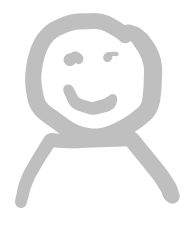
\includegraphics[width = 0.6 cm]{../assets/images/agents/avatar_rand5_gray}};
\node (agent2) at (9.2, 5) {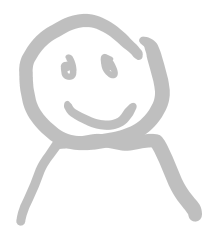
\includegraphics[width = 0.6 cm]{../assets/images/agents/avatar_rand4_gray}};
\node (agent3) at (8.8, 2.5) {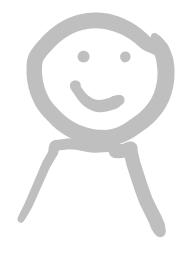
\includegraphics[width = 0.6 cm]{../assets/images/agents/avatar_rand3_gray}};

\node (key1) at (agentg.east) {
\includegraphics[width = 0.3 cm]{../assets/images/key_gray}};
\node[xshift=0.3 cm] (key2) at (agentg.east) {
\includegraphics[width = 0.3 cm]{../assets/images/key_gray}};
\node[xshift=0.6 cm] (key3) at (agentg.east) {
\includegraphics[width = 0.3 cm]{../assets/images/key_gray}};

\node (agent4) at (1, -1) {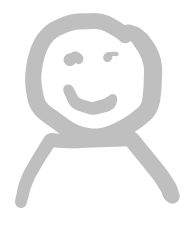
\includegraphics[width = 0.6 cm]{../assets/images/agents/avatar_rand5_gray}};
\node (agent5) at (4.1, -1.7) {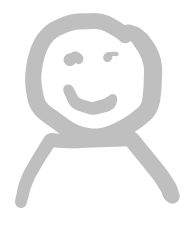
\includegraphics[width = 0.6 cm]{../assets/images/agents/avatar_rand5_gray}};

\node (key4) at (agent4.west) {
\includegraphics[width = 0.3 cm]{../assets/images/key_gray}};
\node (key5) at (agent5.west) {
\includegraphics[width = 0.3 cm]{../assets/images/key_gray}};

\color{lightgray}
\draw[<->, thick, dashed]	(agentg.north) -- (agent1.south);
\draw[<->, thick, dashed]	(agentg.north east) -- (agent2.south west);
\draw[<->, thick, dashed]	(agentg.south east) -- (agent3.north west);

\draw[<->, thick, dashed]	(agentd.south west) -- (agent4.east);
\draw[<->, thick, dashed]	(agentd.south east) -- (agent5.north west);

%TRX 
\only<1->{
\node (TRXa) at (agenta.north west) {\tiny{TRX}};
}
\only<2->{
\node (TRXc) at (agentc.north) {\tiny{TRX}};
\node (TRXb) at (agentb.south west) {\tiny{TRX}};
\node (TRXe) at (agente.north) {\tiny{TRX}};
}
\only<3->{
\node (TRXg) at (agentg.north west) {\tiny{TRX}};
\node (TRXf) at (agentf.north west) {\tiny{TRX}};
\node (TRXd) at (agentd.south) {\tiny{TRX}};
}
\only<4->{
\node (TRXh) at (agenth.south east) {\tiny{TRX}};
}
	\end{tikzpicture}
\end{figure}
\end{frame}
%%%	


%%%
\begin{frame}{From Transactions to Blocks}
	\begin{enumerate}
		\item<1-> Node sends his transaction to the connected peers.
		\item<1-> Each node verifies the received transaction
			\begin{itemize}
				\item<1-> Inputs, Outputs, Signatures
			\end{itemize}			 
		\item<1-> If the transaction is valid, it is \dots
			\begin{itemize}
				\item<1-> \dots forwarded to respective peers.
				\item<1-> \dots stored in own transaction mempool
			\end{itemize}
	\end{enumerate}	
	\vspace{1em}
	\uncover<1->{Miners will take the transactions (with the highest fees) from their mempool and form a block, but how is this done?}
\end{frame}
%%%

%%%
\begin{frame}{Merkle Root}
	\begin{columns}
	\column{0.7\textwidth}
		\begin{figure}
			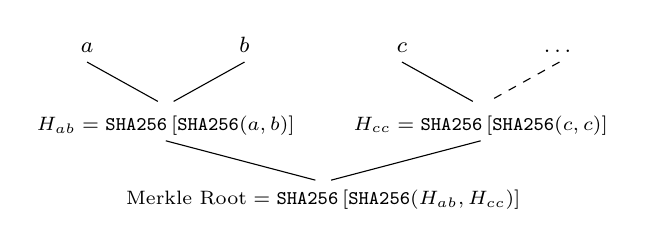
\begin{tikzpicture}[domain=-6:6,scale=1, every node/.style={scale=1}]

% 1st level
\draw[color=black, -] (-5,5) -- (-4.1,4.5); 
\draw (-5,5)node[above]{\footnotesize{$a$}};
\draw[color=black, -] (-3,5) -- (-3.9,4.5);
\draw (-3,5)node[above]{\footnotesize{$b$}};

\draw[color=black, -] (-1,5) -- (-0.1,4.5);
\draw (-1,5)node[above]{\footnotesize{$c$}};
\draw[color=black, -, dashed] (1,5) -- (0.1,4.5);
\draw (1,5)node[above]{\footnotesize{$\dots$}};

% 2nd level
\draw[color=black, -] (-4,4) -- (-2.1,3.5);
\draw (-4,3.95)node[above]{\scriptsize{$H_{ab}=\texttt{SHA256}\left[\texttt{SHA256}(a,b)\right]$}};
\draw[color=black, -] (0,4) -- (-1.9,3.5);
\draw (0,3.95)node[above]{\scriptsize{$H_{cc}=\texttt{SHA256}\left[\texttt{SHA256}(c,c)\right]$}};

\draw (-2,3.5)node[below]{\scriptsize{$\text{Merkle Root}={}\texttt{SHA256}\left[\texttt{SHA256}(H_{ab},H_{cc})\right]$}};
\end{tikzpicture}
		\end{figure}
		\begin{itemize}
			\item Represents all transactions of the block in the form of a compact 256-bit entry.
			\item Guarantees that the transaction data of a block cannot be modified unnoticed.
		\end{itemize}
	\column{0.3\textwidth}
		\begin{figure}
			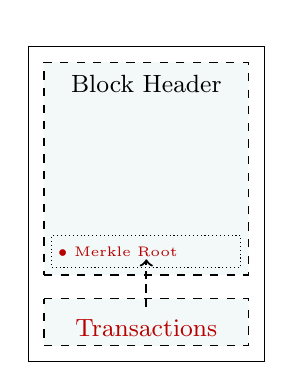
\begin{tikzpicture}[domain=-8:8,scale=1, every node/.style={scale=1}]
  
  % Block 
  \draw[fill=white] (-2,0) -- (1,0) -- (1,4) -- (-2,4) node[above,midway] {{}} -- (-2,0);
  
    % header
    \draw[dashed, fill=highlight!15] (-1.8,1.1) -- (0.8,1.1) -- (0.8,3.8) -- (-1.8,3.8) -- (-1.8,1.1);    
    %\draw[color=black, ->, dashed] (0.8,2.45) -- (2.35,2.8);
    \draw[color=black] plot (-0.5,3.3)    node[above] {\small{Block Header}};
    \draw[densely dotted] (-1.7,1.2) -- (0.7,1.2) -- (0.7,1.6) -- (-1.7,1.6) -- (-1.7,1.2);   
    
    % Transactions
    \draw[dashed, fill=highlight!15] (-1.8,0.8) -- (0.8,0.8) -- (0.8,0.2) -- (-1.8,0.2) node[above,midway, color=focus] {\small{Transactions}} -- (-1.8,0.8);
    \draw[color=black, ->, densely dashed,thick] (-0.5,0.7) -- (-0.5,1.3);
    
    %\node[right] at (-1.75,3.15) {\tiny{$\bullet$ Version}} ;
    %\node[right] at (-1.75,2.8) {\tiny{$\bullet$ Reference}} ;
    %\node[right] at (-1.75,2.45) {\tiny{$\bullet$ Timestamp}} ;
    %\node[right] at (-1.75,2.1) {\tiny{$\bullet$ Treshold}} ;
    %\node[right] at (-1.75,1.75) {\tiny{$\bullet$ Nonce}} ;
    \node[right, color=focus] at (-1.75,1.4) {\tiny{$\bullet$ Merkle Root}} ;
  
\end{tikzpicture}
		\end{figure}
	\end{columns}
\end{frame}
%%%


%%%
\begin{frame}{Version, Reference \& Timestamp}
	\begin{columns}
	\column{0.7\textwidth}
		\begin{itemize}
			\item \textbf{Version:} Followed ruleset of block creation, implicates validation rules.
			\item \textbf{Reference:} Hash value of predecessor block header $\rightarrow$ Basis for chain structure.
			\item \textbf{Timestamp:} At least median timestamp of the previous eleven blocks, not more than two hours in the future at the time of inclusion in the blockchain. 
		\end{itemize}
	\column{0.3\textwidth}
		\begin{figure}
			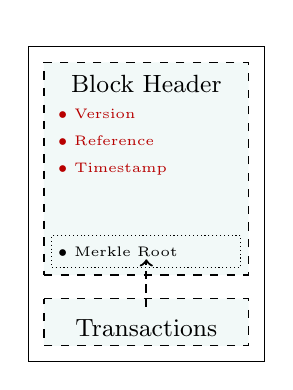
\begin{tikzpicture}[domain=-8:8,scale=1, every node/.style={scale=1}]
  
  % Block 
  \draw[fill=white] (-2,0) -- (1,0) -- (1,4) -- (-2,4) node[above,midway] {{}} -- (-2,0);
  
    % header
    \draw[dashed, fill=highlight!15] (-1.8,1.1) -- (0.8,1.1) -- (0.8,3.8) -- (-1.8,3.8) -- (-1.8,1.1);    
    %\draw[color=black, ->, dashed] (0.8,2.45) -- (2.35,2.8);
    \draw[color=black] plot (-0.5,3.3)    node[above] {\small{Block Header}};
    \draw[densely dotted] (-1.7,1.2) -- (0.7,1.2) -- (0.7,1.6) -- (-1.7,1.6) -- (-1.7,1.2);   
    
    % Transactions
    \draw[dashed, fill=highlight!15] (-1.8,0.8) -- (0.8,0.8) -- (0.8,0.2) -- (-1.8,0.2) node[above,midway] {\small{Transactions}} -- (-1.8,0.8);
    \draw[color=black, ->, densely dashed,thick] (-0.5,0.7) -- (-0.5,1.3);
    
    \node[right, color=focus] at (-1.75,3.15) {\tiny{$\bullet$ Version}} ;
    \node[right, color=focus] at (-1.75,2.8) {\tiny{$\bullet$ Reference}} ;
    \node[right, color=focus] at (-1.75,2.45) {\tiny{$\bullet$ Timestamp}} ;
    %\node[right] at (-1.75,2.1) {\tiny{$\bullet$ Treshold}} ;
    %\node[right] at (-1.75,1.75) {\tiny{$\bullet$ Nonce}} ;
    \node[right] at (-1.75,1.4) {\tiny{$\bullet$ Merkle Root}} ;
  
\end{tikzpicture}
		\end{figure}
	\end{columns}
\end{frame}
%%%


%%%
\begin{frame}{Threshold and Nonce}
	\begin{columns}
	\column{0.7\textwidth}
		\begin{itemize}
			\item \textbf{Threshold:} Shows the maximum hash value a block header may have in order to be considered valid by the network and become part of the blockchain
			\item \textbf{Nonce:} Primary source of variation in block creation. Ensures that blocks with otherwise equivalent content can nevertheless have different hash values.
		\end{itemize}
	\column{0.3\textwidth}
		\begin{figure}
			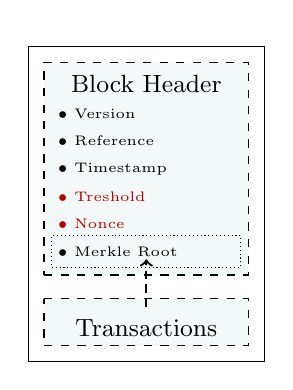
\begin{tikzpicture}[domain=-8:8,scale=1, every node/.style={scale=1}]
  
  % Block 
  \draw[fill=white] (-2,0) -- (1,0) -- (1,4) -- (-2,4) node[above,midway] {{}} -- (-2,0);
  
    % header
    \draw[dashed, fill=highlight!15] (-1.8,1.1) -- (0.8,1.1) -- (0.8,3.8) -- (-1.8,3.8) -- (-1.8,1.1);    
    %\draw[color=black, ->, dashed] (0.8,2.45) -- (2.35,2.8);
    \draw[color=black] plot (-0.5,3.3)    node[above] {\small{Block Header}};
    \draw[densely dotted] (-1.7,1.2) -- (0.7,1.2) -- (0.7,1.6) -- (-1.7,1.6) -- (-1.7,1.2);   
    
    % Transactions
    \draw[dashed, fill=highlight!15] (-1.8,0.8) -- (0.8,0.8) -- (0.8,0.2) -- (-1.8,0.2) node[above,midway] {\small{Transactions}} -- (-1.8,0.8);
    \draw[color=black, ->, densely dashed,thick] (-0.5,0.7) -- (-0.5,1.3);
    
    \node[right] at (-1.75,3.15) {\tiny{$\bullet$ Version}} ;
    \node[right] at (-1.75,2.8) {\tiny{$\bullet$ Reference}} ;
    \node[right] at (-1.75,2.45) {\tiny{$\bullet$ Timestamp}} ;
    \node[right, color=focus] at (-1.75,2.1) {\tiny{$\bullet$ Treshold}} ;
    \node[right, color=focus] at (-1.75,1.75) {\tiny{$\bullet$ Nonce}} ;
    \node[right] at (-1.75,1.4) {\tiny{$\bullet$ Merkle Root}} ;
  
\end{tikzpicture}
		\end{figure}
	\end{columns}
\end{frame}
%%%


%%%
\begin{frame}{Meta Data}
	\begin{columns}
	\column{0.5\textwidth}
		\begin{itemize}
			\item \textbf{Time, Mediantime:} Timestamped data
			\item \textbf{Difficulty:} Proof of work
			\item \textbf{Chainwork:} Total number of hashes that are expected to have been necessary to produce the current chain
			\item \textbf{Number of transactions, Size:} Scalability
		\end{itemize}
	\column{0.5\textwidth}
		\begin{figure}
			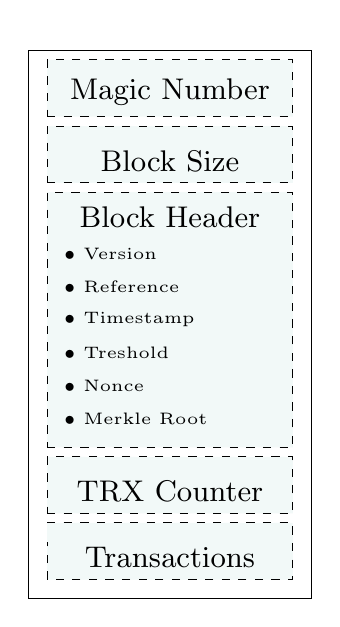
\begin{tikzpicture}[domain=-8:8,scale=1.2, every node/.style={scale=1.2}]
  				  % Block 
  \draw[fill=white] (-2,0.2) -- (1,0.2) -- (1,6) -- (-2,6) node[above,midway] {{}} -- (-2,0.2);
  
  % Magic No
  \draw[dashed, fill=highlight!15] (-1.8,5.3) -- (0.8,5.3) node[above, midway] {\alert{\small{Magic Number}}}-- (0.8,5.9) -- (-1.8,5.9) -- (-1.8,5.3); 
  
  % Blocksize
  \draw[dashed, fill=highlight!15] (-1.8,4.6) -- (0.8,4.6)  node[above, midway] {\alert{\small{Block Size}}} -- (0.8,5.2) -- (-1.8,5.2) --(-1.8,4.6); 
  
  % Header
    \draw[dashed, fill=highlight!15] (-1.8,1.8) -- (0.8,1.8) -- (0.8,4.5) -- (-1.8,4.5) -- (-1.8,1.8);    
    %\draw[color=black, ->, dashed] (0.8,2.45) -- (2.35,2.8);
    \draw[color=black] plot (-0.5,4)    node[above] {\small{Block Header}};
    %\draw[densely dotted] (-1.7,1.9) -- (0.7,1.9) -- (0.7,2.3) -- (-1.7,2.3) -- (-1.7,1.9);
    
  % Transaction Counter
     \draw[dashed, fill=highlight!15] (-1.8,1.1) -- (0.8,1.1) node[above, midway] {\alert{\small{TRX Counter}}} -- (0.8,1.7) -- (-1.8,1.7) -- (-1.8,1.1) ;
     %\draw[color=black] plot (-0.5,1.4)    node[above] {\small{TRX Counter}}; 
    
  % Transactions
    \draw[dashed, fill=highlight!15] (-1.8,1) -- (0.8,1) -- (0.8,0.4) -- (-1.8,0.4) node[above,midway] {\small{Transactions}} -- (-1.8,0.8);
    %\draw[color=black, ->, densely dashed,thick] (-0.5,0.7) -- (-0.5,1.3);
    
    \node[right] at (-1.75,3.85) {\tiny{$\bullet$ Version}} ;
    \node[right] at (-1.75,3.5) {\tiny{$\bullet$ Reference}} ;
    \node[right] at (-1.75,3.15) {\tiny{$\bullet$ Timestamp}} ;
    \node[right] at (-1.75,2.8) {\tiny{$\bullet$ Treshold}} ;
    \node[right] at (-1.75,2.45) {\tiny{$\bullet$ Nonce}} ;
    \node[right] at (-1.75,2.1) {\tiny{$\bullet$ Merkle Root}} ;
  			\end{tikzpicture}
			\end{figure}
	\end{columns}
\end{frame}
%%%


%%%
\begin{frame}{Block Height and -Depth}
	\begin{figure}
		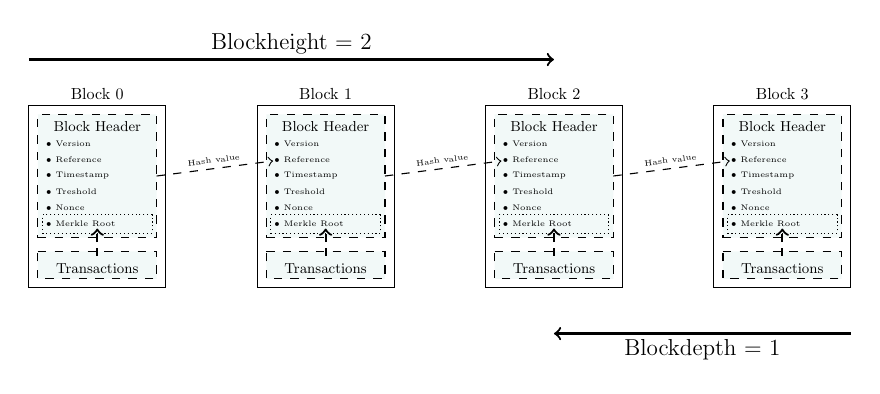
\begin{tikzpicture}[domain=-8:8,scale=0.58, every node/.style={scale=0.58}]

% Block 0
  \draw[fill=white] (-6,0) -- (-3,0) -- (-3,4) -- (-6,4) node[above,midway] {{Block 0}} -- (-6,0);
  
    % header
    \draw[dashed, fill=highlight!15] (-5.8,1.1) -- (-3.2,1.1) -- (-3.2,3.8) -- (-5.8,3.8) -- (-5.8,1.1);    
    \draw[color=black] plot (-4.5,3.3)    node[above] {\small{Block Header}};
    \draw[densely dotted] (-5.7,1.2) -- (-3.3,1.2) -- (-3.3,1.6) -- (-5.7,1.6) -- (-5.7,1.2);   
    
    % Transactions
    \draw[dashed, fill=highlight!15] (-5.8,0.8) -- (-3.2,0.8) -- (-3.2,0.2) -- (-5.8,0.2) node[above,midway] {\small{Transactions}} -- (-5.8,0.8);
    \draw[color=black, ->, densely dashed,thick] (-4.5,0.7) -- (-4.5,1.3);
    
    \node[right] at (-5.75,3.15) {\tiny{$\bullet$ Version}} ;
    \node[right] at (-5.75,2.8) {\tiny{$\bullet$ Reference}} ;
    \node[right] at (-5.75,2.45) {\tiny{$\bullet$ Timestamp}} ;
    \node[right] at (-5.75,2.1) {\tiny{$\bullet$ Treshold}} ;
    \node[right] at (-5.75,1.75) {\tiny{$\bullet$ Nonce}} ;
    \node[right] at (-5.75,1.4) {\tiny{$\bullet$ Merkle Root}} ;
  
   % Block 1
  \draw[fill=white] (-1,0) -- (2,0) -- (2,4) -- (-1,4) node[above,midway] {{Block 1}} -- (-1,0);
  
    % header
    \draw[dashed, fill=highlight!15] (-0.8,1.1) -- (1.8,1.1) -- (1.8,3.8) -- (-0.8,3.8) -- (-0.8,1.1);    
    \draw[color=black] plot (0.5,3.3)    node[above] {\small{Block Header}};
    \draw[densely dotted] (-0.7,1.2) -- (1.7,1.2) -- (1.7,1.6) -- (-0.7,1.6) -- (-0.7,1.2);   
    
    % Transactions
    \draw[dashed, fill=highlight!15] (-0.8,0.8) -- (1.8,0.8) -- (1.8,0.2) -- (-0.8,0.2) node[above,midway] {\small{Transactions}} -- (-0.8,0.8);
    \draw[color=black, ->, densely dashed,thick] (0.5,0.7) -- (0.5,1.3);
    
    \node[right] at (-0.75,3.15) {\tiny{$\bullet$ Version}} ;
    \node[right] at (-0.75,2.8) {\tiny{$\bullet$ Reference}} ;
    \node[right] at (-0.75,2.45) {\tiny{$\bullet$ Timestamp}} ;
    \node[right] at (-0.75,2.1) {\tiny{$\bullet$ Treshold}} ;
    \node[right] at (-0.75,1.75) {\tiny{$\bullet$ Nonce}} ;
    \node[right] at (-0.75,1.4) {\tiny{$\bullet$ Merkle Root}} ;
  
  
  
  % Block 2
 \draw[fill=white] (4,0) -- (7,0) -- (7,4) -- (4,4) node[above,midway] {{Block 2}} -- (4,0);
  
    % header
    \draw[dashed, fill=highlight!15] (4.2,1.1) -- (6.8,1.1) -- (6.8,3.8) -- (4.2,3.8) -- (4.2,1.1);    
    %\draw[color=black, ->, dashed] (4.8,2.45) -- (6.35,2.8);
    \draw[color=black] plot (5.5,3.3)    node[above] {\small{Block Header}};
    \draw[densely dotted] (4.3,1.2) -- (6.7,1.2) -- (6.7,1.6) -- (4.3,1.6) -- (4.3,1.2);   
    
    % Transactions
    \draw[dashed, fill=highlight!15] (4.2,0.8) -- (6.8,0.8) -- (6.8,0.2) -- (4.2,0.2) node[above,midway] {\small{Transactions}} -- (4.2,0.8);
    \draw[color=black, ->, densely dashed,thick] (5.5,0.7) -- (5.5,1.3);
    
    \node[right] at (4.25,3.15) {\tiny{$\bullet$ Version}} ;
    \node[right] at (4.25,2.8) {\tiny{$\bullet$ Reference}} ;
    \node[right] at (4.25,2.45) {\tiny{$\bullet$ Timestamp}} ;
    \node[right] at (4.25,2.1) {\tiny{$\bullet$ Treshold}} ;
    \node[right] at (4.25,1.75) {\tiny{$\bullet$ Nonce}} ;
    \node[right] at (4.25,1.4) {\tiny{$\bullet$ Merkle Root}} ;  
    
  % Block 3
 \draw[fill=white] (9,0) -- (12,0) -- (12,4) -- (9,4) node[above,midway] {{Block 3}} -- (9,0);
  
    % header
    \draw[dashed, fill=highlight!15] (9.2,1.1) -- (11.8,1.1) -- (11.8,3.8) -- (9.2,3.8) -- (9.2,1.1);    
    %\draw[color=black, ->, dashed] (4.8,2.45) -- (6.35,2.8);
    \draw[color=black] plot (10.5,3.3)    node[above] {\small{Block Header}};
    \draw[densely dotted] (9.3,1.2) -- (11.7,1.2) -- (11.7,1.6) -- (9.3,1.6) -- (9.3,1.2);   
    
    % Transactions
    \draw[dashed, fill=highlight!15] (9.2,0.8) -- (11.8,0.8) -- (11.8,0.2) -- (9.2,0.2) node[above,midway] {\small{Transactions}} -- (9.2,0.8);
    \draw[color=black, ->, densely dashed,thick] (10.5,0.7) -- (10.5,1.3);
    
    \node[right] at (9.25,3.15) {\tiny{$\bullet$ Version}} ;
    \node[right] at (9.25,2.8) {\tiny{$\bullet$ Reference}} ;
    \node[right] at (9.25,2.45) {\tiny{$\bullet$ Timestamp}} ;
    \node[right] at (9.25,2.1) {\tiny{$\bullet$ Treshold}} ;
    \node[right] at (9.25,1.75) {\tiny{$\bullet$ Nonce}} ;
    \node[right] at (9.25,1.4) {\tiny{$\bullet$ Merkle Root}} ;  


\draw[color=black, ->, dashed] (-3.2,2.45) -- (-0.65,2.78) node[above,midway,rotate=7.5]{\tiny{Hash value}} ;%node[below,midway,rotate=7.5]{\tiny{\texttt{SHA256[SHA256()]}}};
\draw[color=black, ->, dashed] (1.8,2.45) -- (4.35,2.78) node[above,midway,rotate=7.5]{\tiny{Hash value}} ;
\draw[color=black, ->, dashed] (6.8,2.45) -- (9.35,2.78) node[above,midway,rotate=7.5]{\tiny{Hash value}} ;

\draw[->,thick] (-6,5) -- (5.5,5) node[above,midway]{\Large{Blockheight = 2}};
\draw[->,thick] (12,-1) -- (5.5,-1) node[below,midway]{\Large{Blockdepth = 1}};

\end{tikzpicture}
	\end{figure}
\textbf{Block Identification:}
	\begin{itemize}
 		\item Block Height (static, not unique in case of fork)
 		\item Block Depth (dynamic)
 		\item Block Header hash value / Block ID (static)
	\end{itemize}
\end{frame}
%%%


%%%
\begin{frame}{The Domino Effect 1}
	\begin{figure}
		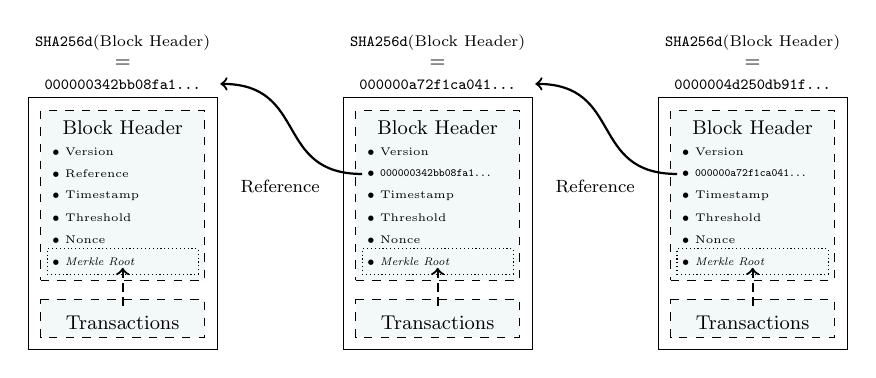
\begin{tikzpicture}[domain=-8:8,scale=0.8, every node/.style={scale=0.8}]

% Block 0
  \draw[fill=white] (-6,0) -- (-3,0) -- (-3,4) -- (-6,4) node[above=0.5cm,midway]{\scriptsize{\texttt{SHA256d}(\text{Block Header})}} node[above=0.29cm,midway]{\small{=}} node[above=0cm,midway]{\scriptsize{\texttt{000000342bb08fa1\dots}}} -- (-6,0);
  
    % header
    \draw[dashed, fill=highlight!15] (-5.8,1.1) -- (-3.2,1.1) -- (-3.2,3.8) -- (-5.8,3.8) -- (-5.8,1.1);    
    \draw[color=black] plot (-4.5,3.3)    node[above] {\small{Block Header}};
    \draw[densely dotted] (-5.7,1.2) -- (-3.3,1.2) -- (-3.3,1.6) -- (-5.7,1.6) -- (-5.7,1.2);   
    
    % Transactions
    \draw[dashed, fill=highlight!15] (-5.8,0.8) -- (-3.2,0.8) -- (-3.2,0.2) -- (-5.8,0.2) node[above,midway] {\small{Transactions}} -- (-5.8,0.8);
    \draw[color=black, ->, densely dashed,thick] (-4.5,0.7) -- (-4.5,1.3);
    
    \node[right] at (-5.75,3.15) {\tiny{$\bullet$ Version}} ;
    \node[right] at (-5.75,2.8) {\tiny{$\bullet$ Reference}} ;
    \node[right] at (-5.75,2.45) {\tiny{$\bullet$ Timestamp}} ;
    \node[right] at (-5.75,2.1) {\tiny{$\bullet$ Threshold}} ;
    \node[right] at (-5.75,1.75) {\tiny{$\bullet$ Nonce}} ;
    \node[right] at (-5.75,1.4) {\tiny{$\bullet$ \textit{Merkle Root}}} ;
  
   % Block 1
  \draw[fill=white] (-1,0) -- (2,0) -- (2,4) -- (-1,4) node[above=0.5cm,midway]{\scriptsize{\texttt{SHA256d}(\text{Block Header})}} node[above=0.29cm,midway]{\small{=}} node[above=0cm,midway]{\scriptsize{\texttt{000000a72f1ca041\dots}}} -- (-1,0);
  
    % header
    \draw[dashed, fill=highlight!15] (-0.8,1.1) -- (1.8,1.1) -- (1.8,3.8) -- (-0.8,3.8) -- (-0.8,1.1);    
    \draw[color=black] plot (0.5,3.3)    node[above] {\small{Block Header}};
    \draw[densely dotted] (-0.7,1.2) -- (1.7,1.2) -- (1.7,1.6) -- (-0.7,1.6) -- (-0.7,1.2);   
    
    % Transactions
    \draw[dashed, fill=highlight!15] (-0.8,0.8) -- (1.8,0.8) -- (1.8,0.2) -- (-0.8,0.2) node[above,midway] {\small{Transactions}} -- (-0.8,0.8);
    \draw[color=black, ->, densely dashed,thick] (0.5,0.7) -- (0.5,1.3);
    
    \node[right] at (-0.75,3.15) {\tiny{$\bullet$ Version}} ;
    \node[right] at (-0.75,2.8) {\tiny{$\bullet$ \texttt{000000342bb08fa1\dots}}} ;
    \node[right] at (-0.75,2.45) {\tiny{$\bullet$ Timestamp}} ;
    \node[right] at (-0.75,2.1) {\tiny{$\bullet$ Threshold}} ;
    \node[right] at (-0.75,1.75) {\tiny{$\bullet$ Nonce}} ;
    \node[right] at (-0.75,1.4) {\tiny{$\bullet$ \textit{Merkle Root}}} ;
    
  % Block 2
 \draw[fill=white] (4,0) -- (7,0) -- (7,4) -- (4,4) node[above=0.5cm,midway]{\scriptsize{\texttt{SHA256d}(\text{Block Header})}} node[above=0.29cm,midway]{\small{=}} node[above=0cm,midway]{\scriptsize{\texttt{0000004d250db91f\dots}}} -- (4,0);
  
    % header
    \draw[dashed, fill=highlight!15] (4.2,1.1) -- (6.8,1.1) -- (6.8,3.8) -- (4.2,3.8) -- (4.2,1.1);    
    %\draw[color=black, ->, dashed] (4.8,2.45) -- (6.35,2.8);
    \draw[color=black] plot (5.5,3.3)    node[above] {\small{Block Header}};
    \draw[densely dotted] (4.3,1.2) -- (6.7,1.2) -- (6.7,1.6) -- (4.3,1.6) -- (4.3,1.2);   
    
    % Transactions
    \draw[dashed, fill=highlight!15] (4.2,0.8) -- (6.8,0.8) -- (6.8,0.2) -- (4.2,0.2) node[above,midway] {\small{Transactions}} -- (4.2,0.8);
    \draw[color=black, ->, densely dashed,thick] (5.5,0.7) -- (5.5,1.3);
    
    \node[right] at (4.25,3.15) {\tiny{$\bullet$ Version}} ;
    \node[right] at (4.25,2.8) {\tiny{$\bullet$ \texttt{000000a72f1ca041\dots}}} ;
    \node[right] at (4.25,2.45) {\tiny{$\bullet$ Timestamp}} ;
    \node[right] at (4.25,2.1) {\tiny{$\bullet$ Threshold}} ;
    \node[right] at (4.25,1.75) {\tiny{$\bullet$ Nonce}} ;
    \node[right] at (4.25,1.4) {\tiny{$\bullet$ \textit{Merkle Root}}} ;  
    


%\draw[color=black, ->, dashed] (-3.2,2.45) -- (-0.65,2.78) node[above,midway,rotate=7.5]{\tiny{Hashwert}} ;%node[below,midway,rotate=7.5]{\tiny{\texttt{SHA256[SHA256()]}}};
%\draw[color=black, ->, dashed] (1.8,2.45) -- (4.35,2.78) node[above,midway,rotate=7.5]{\tiny{Hashwert}} ;
%\draw[color=black, ->, dashed] (6.8,2.45) -- (9.35,2.78) node[above,midway,rotate=7.5]{\tiny{Hashwert}} ;

\draw[shorten >=0.28cm,shorten <=0.28cm,thick,<-,color=black] (-3.3,4.22) to[out = 0, in = 180, distance=50] (-0.35,2.79);
\draw[color=white!0](-2,2.6)--(-2,2.6)node[rotate=0,color=black]{\footnotesize{Reference}};
\draw[shorten >=0.28cm,shorten <=0.28cm,thick,<-] (1.7,4.22) to[out = 0, in = 180, distance=50] (4.65,2.79);
\draw[color=white!0](3,2.6)--(3,2.6)node[rotate=0,color=black]{\footnotesize{Reference}};

%\draw[thick] (-2.2,3.25)--(-1.8,4.25);
%\draw[thick] (-2,3)--(-1.6,4);

\end{tikzpicture}

	\end{figure}
\end{frame}
%%%


%%%
\begin{frame}{The Domino Effect 2}
	\begin{figure}
		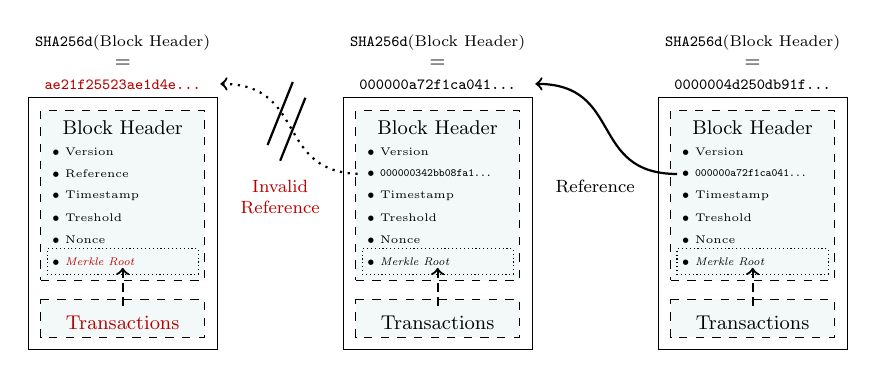
\begin{tikzpicture}[domain=-8:8,scale=0.8, every node/.style={scale=0.8}]

% Block 0
  \draw[fill=white] (-6,0) -- (-3,0) -- (-3,4) -- (-6,4) node[above=0.5cm,midway]{\scriptsize{\texttt{SHA256d}(\text{Block Header})}} node[above=0.29cm,midway]{\small{=}} node[above=0cm,midway,color=focus]{\scriptsize{\texttt{ae21f25523ae1d4e\dots}}} -- (-6,0);
  
    % header
    \draw[dashed, fill=highlight!15] (-5.8,1.1) -- (-3.2,1.1) -- (-3.2,3.8) -- (-5.8,3.8) -- (-5.8,1.1);    
    \draw[color=black] plot (-4.5,3.3)    node[above] {\small{Block Header}};
    \draw[densely dotted] (-5.7,1.2) -- (-3.3,1.2) -- (-3.3,1.6) -- (-5.7,1.6) -- (-5.7,1.2);   
    
    % Transactions
    \draw[dashed, fill=highlight!15] (-5.8,0.8) -- (-3.2,0.8) -- (-3.2,0.2) -- (-5.8,0.2) node[above,midway] {\small{\color{focus}Transactions\color{black}}} -- (-5.8,0.8);
    \draw[color=black, ->, densely dashed,thick] (-4.5,0.7) -- (-4.5,1.3);
    
    \node[right] at (-5.75,3.15) {\tiny{$\bullet$ Version}} ;
    \node[right] at (-5.75,2.8) {\tiny{$\bullet$ Reference}} ;
    \node[right] at (-5.75,2.45) {\tiny{$\bullet$ Timestamp}} ;
    \node[right] at (-5.75,2.1) {\tiny{$\bullet$ Treshold}} ;
    \node[right] at (-5.75,1.75) {\tiny{$\bullet$ Nonce}} ;
    \node[right] at (-5.75,1.4) {\tiny{$\bullet$ \color{focus}\textit{Merkle Root}}} ;
  
   % Block 1
  \draw[fill=white] (-1,0) -- (2,0) -- (2,4) -- (-1,4) node[above=0.5cm,midway]{\scriptsize{\texttt{SHA256d}(\text{Block Header})}} node[above=0.29cm,midway]{\small{=}} node[above=0cm,midway]{\scriptsize{\texttt{000000a72f1ca041\dots}}} -- (-1,0);
  
    % header
    \draw[dashed, fill=highlight!15] (-0.8,1.1) -- (1.8,1.1) -- (1.8,3.8) -- (-0.8,3.8) -- (-0.8,1.1);    
    \draw[color=black] plot (0.5,3.3)    node[above] {\small{Block Header}};
    \draw[densely dotted] (-0.7,1.2) -- (1.7,1.2) -- (1.7,1.6) -- (-0.7,1.6) -- (-0.7,1.2);   
    
    % Transactions
    \draw[dashed, fill=highlight!15] (-0.8,0.8) -- (1.8,0.8) -- (1.8,0.2) -- (-0.8,0.2) node[above,midway] {\small{Transactions}} -- (-0.8,0.8);
    \draw[color=black, ->, densely dashed,thick] (0.5,0.7) -- (0.5,1.3);
    
    \node[right] at (-0.75,3.15) {\tiny{$\bullet$ Version}} ;
    \node[right] at (-0.75,2.8) {\tiny{$\bullet$ \texttt{000000342bb08fa1\dots}}} ;
    \node[right] at (-0.75,2.45) {\tiny{$\bullet$ Timestamp}} ;
    \node[right] at (-0.75,2.1) {\tiny{$\bullet$ Treshold}} ;
    \node[right] at (-0.75,1.75) {\tiny{$\bullet$ Nonce}} ;
    \node[right] at (-0.75,1.4) {\tiny{$\bullet$ \textit{Merkle Root}}} ;
    
  % Block 2
 \draw[fill=white] (4,0) -- (7,0) -- (7,4) -- (4,4) node[above=0.5cm,midway]{\scriptsize{\texttt{SHA256d}(\text{Block Header})}} node[above=0.29cm,midway]{\small{=}} node[above=0cm,midway]{\scriptsize{\texttt{0000004d250db91f\dots}}} -- (4,0);
  
    % header
    \draw[dashed, fill=highlight!15] (4.2,1.1) -- (6.8,1.1) -- (6.8,3.8) -- (4.2,3.8) -- (4.2,1.1);    
    %\draw[color=black, ->, dashed] (4.8,2.45) -- (6.35,2.8);
    \draw[color=black] plot (5.5,3.3)    node[above] {\small{Block Header}};
    \draw[densely dotted] (4.3,1.2) -- (6.7,1.2) -- (6.7,1.6) -- (4.3,1.6) -- (4.3,1.2);   
    
    % Transactions
    \draw[dashed, fill=highlight!15] (4.2,0.8) -- (6.8,0.8) -- (6.8,0.2) -- (4.2,0.2) node[above,midway] {\small{Transactions}} -- (4.2,0.8);
    \draw[color=black, ->, densely dashed,thick] (5.5,0.7) -- (5.5,1.3);
    
    \node[right] at (4.25,3.15) {\tiny{$\bullet$ Version}} ;
    \node[right] at (4.25,2.8) {\tiny{$\bullet$ \texttt{000000a72f1ca041\dots}}} ;
    \node[right] at (4.25,2.45) {\tiny{$\bullet$ Timestamp}} ;
    \node[right] at (4.25,2.1) {\tiny{$\bullet$ Treshold}} ;
    \node[right] at (4.25,1.75) {\tiny{$\bullet$ Nonce}} ;
    \node[right] at (4.25,1.4) {\tiny{$\bullet$ \textit{Merkle Root}}} ;  
    


%\draw[color=black, ->, dashed] (-3.2,2.45) -- (-0.65,2.78) node[above,midway,rotate=7.5]{\tiny{Hashwert}} ;%node[below,midway,rotate=7.5]{\tiny{\texttt{SHA256[SHA256()]}}};
%\draw[color=black, ->, dashed] (1.8,2.45) -- (4.35,2.78) node[above,midway,rotate=7.5]{\tiny{Hashwert}} ;
%\draw[color=black, ->, dashed] (6.8,2.45) -- (9.35,2.78) node[above,midway,rotate=7.5]{\tiny{Hashwert}} ;

\draw[shorten >=0.28cm,shorten <=0.28cm,thick,<-,dotted,color=black] (-3.3,4.22) to[out = 0, in = 180, distance=50] (-0.35,2.79);
\draw[color=white!0](-2,2.6)--(-2,2.6)node[rotate=0,color=focus]{\footnotesize{Invalid}}node[below=0.1cm,rotate=0,color=focus]{\footnotesize{Reference}};
\draw[shorten >=0.28cm,shorten <=0.28cm,thick,<-] (1.7,4.22) to[out = 0, in = 180, distance=50] (4.65,2.79);
\draw[color=white!0](3,2.6)--(3,2.6)node[rotate=0,color=black]{\footnotesize{Reference}};

\draw[thick] (-2.2,3.25)--(-1.8,4.25);
\draw[thick] (-2,3)--(-1.6,4);

\end{tikzpicture}
	\end{figure}

		%\item Modification of transactions in Block 0 will change its merkle root and therefore the block header hash, which invalidates the reference to Block 1.
	
\end{frame}
%%%


%%%
\begin{frame}{The Domino Effect 3}
	\begin{figure}
		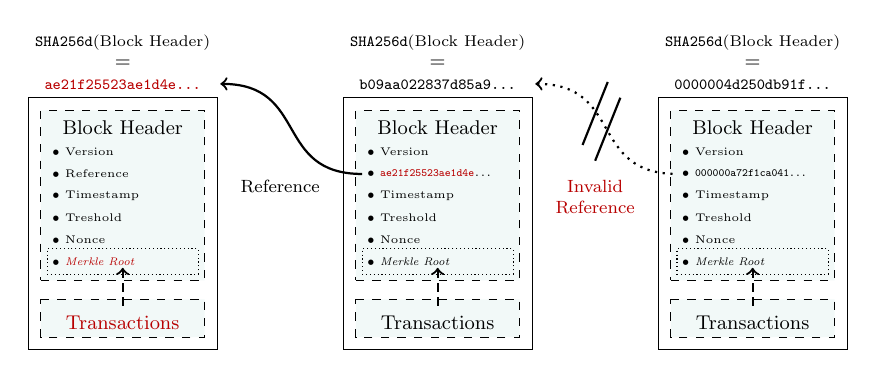
\begin{tikzpicture}[domain=-8:8,scale=0.8, every node/.style={scale=0.8}]

% Block 0
  \draw[fill=white] (-6,0) -- (-3,0) -- (-3,4) -- (-6,4) node[above=0.5cm,midway]{\scriptsize{\texttt{SHA256d}(\text{Block Header})}} node[above=0.29cm,midway]{\small{=}} node[above=0cm,midway,color=focus]{\scriptsize{\texttt{ae21f25523ae1d4e\dots}}} -- (-6,0);
  
    % header
    \draw[dashed, fill=highlight!15] (-5.8,1.1) -- (-3.2,1.1) -- (-3.2,3.8) -- (-5.8,3.8) -- (-5.8,1.1);    
    \draw[color=black] plot (-4.5,3.3)    node[above] {\small{Block Header}};
    \draw[densely dotted] (-5.7,1.2) -- (-3.3,1.2) -- (-3.3,1.6) -- (-5.7,1.6) -- (-5.7,1.2);   
    
    % Transactions
    \draw[dashed, fill=highlight!15] (-5.8,0.8) -- (-3.2,0.8) -- (-3.2,0.2) -- (-5.8,0.2) node[above,midway] {\small{\color{focus}Transactions\color{black}}} -- (-5.8,0.8);
    \draw[color=black, ->, densely dashed,thick] (-4.5,0.7) -- (-4.5,1.3);
    
    \node[right] at (-5.75,3.15) {\tiny{$\bullet$ Version}} ;
    \node[right] at (-5.75,2.8) {\tiny{$\bullet$ Reference}} ;
    \node[right] at (-5.75,2.45) {\tiny{$\bullet$ Timestamp}} ;
    \node[right] at (-5.75,2.1) {\tiny{$\bullet$ Treshold}} ;
    \node[right] at (-5.75,1.75) {\tiny{$\bullet$ Nonce}} ;
    \node[right] at (-5.75,1.4) {\tiny{$\bullet$ \color{focus}\textit{Merkle Root}\color{black}}} ;
  
   % Block 1
  \draw[fill=white] (-1,0) -- (2,0) -- (2,4) -- (-1,4) node[above=0.5cm,midway]{\scriptsize{\texttt{SHA256d}(\text{Block Header})}} node[above=0.29cm,midway]{\small{=}} node[above=0cm,midway]{\scriptsize{\texttt{b09aa022837d85a9\dots}}} -- (-1,0);
  
    % header
    \draw[dashed, fill=highlight!15] (-0.8,1.1) -- (1.8,1.1) -- (1.8,3.8) -- (-0.8,3.8) -- (-0.8,1.1);    
    \draw[color=black] plot (0.5,3.3)    node[above] {\small{Block Header}};
    \draw[densely dotted] (-0.7,1.2) -- (1.7,1.2) -- (1.7,1.6) -- (-0.7,1.6) -- (-0.7,1.2);   
    
    % Transactions
    \draw[dashed, fill=highlight!15] (-0.8,0.8) -- (1.8,0.8) -- (1.8,0.2) -- (-0.8,0.2) node[above,midway] {\small{Transactions}} -- (-0.8,0.8);
    \draw[color=black, ->, densely dashed,thick] (0.5,0.7) -- (0.5,1.3);
    
    \node[right] at (-0.75,3.15) {\tiny{$\bullet$ Version}} ;
    \node[right] at (-0.75,2.8) {\tiny{$\bullet$ \texttt{\textcolor{focus}{ae21f25523ae1d4e}\dots}}} ;
    \node[right] at (-0.75,2.45) {\tiny{$\bullet$ Timestamp}} ;
    \node[right] at (-0.75,2.1) {\tiny{$\bullet$ Treshold}} ;
    \node[right] at (-0.75,1.75) {\tiny{$\bullet$ Nonce}} ;
    \node[right] at (-0.75,1.4) {\tiny{$\bullet$ \textit{Merkle Root}}} ;
    
  % Block 2
 \draw[fill=white] (4,0) -- (7,0) -- (7,4) -- (4,4) node[above=0.5cm,midway]{\scriptsize{\texttt{SHA256d}(\text{Block Header})}} node[above=0.29cm,midway]{\small{=}} node[above=0cm,midway]{\scriptsize{\texttt{0000004d250db91f\dots}}} -- (4,0);
  
    % header
    \draw[dashed, fill=highlight!15] (4.2,1.1) -- (6.8,1.1) -- (6.8,3.8) -- (4.2,3.8) -- (4.2,1.1);    
    %\draw[color=black, ->, dashed] (4.8,2.45) -- (6.35,2.8);
    \draw[color=black] plot (5.5,3.3)    node[above] {\small{Block Header}};
    \draw[densely dotted] (4.3,1.2) -- (6.7,1.2) -- (6.7,1.6) -- (4.3,1.6) -- (4.3,1.2);   
    
    % Transactions
    \draw[dashed, fill=highlight!15] (4.2,0.8) -- (6.8,0.8) -- (6.8,0.2) -- (4.2,0.2) node[above,midway] {\small{Transactions}} -- (4.2,0.8);
    \draw[color=black, ->, densely dashed,thick] (5.5,0.7) -- (5.5,1.3);
    
    \node[right] at (4.25,3.15) {\tiny{$\bullet$ Version}} ;
    \node[right] at (4.25,2.8) {\tiny{$\bullet$ \texttt{000000a72f1ca041\dots}}} ;
    \node[right] at (4.25,2.45) {\tiny{$\bullet$ Timestamp}} ;
    \node[right] at (4.25,2.1) {\tiny{$\bullet$ Treshold}} ;
    \node[right] at (4.25,1.75) {\tiny{$\bullet$ Nonce}} ;
    \node[right] at (4.25,1.4) {\tiny{$\bullet$ \textit{Merkle Root}}} ;  
    


%\draw[color=black, ->, dashed] (-3.2,2.45) -- (-0.65,2.78) node[above,midway,rotate=7.5]{\tiny{Hashwert}} ;%node[below,midway,rotate=7.5]{\tiny{\texttt{SHA256[SHA256()]}}};
%\draw[color=black, ->, dashed] (1.8,2.45) -- (4.35,2.78) node[above,midway,rotate=7.5]{\tiny{Hashwert}} ;
%\draw[color=black, ->, dashed] (6.8,2.45) -- (9.35,2.78) node[above,midway,rotate=7.5]{\tiny{Hashwert}} ;

\draw[shorten >=0.28cm,shorten <=0.28cm,thick,<-,color=black] (-3.3,4.22) to[out = 0, in = 180, distance=50] (-0.35,2.79);
\draw[color=white!0](-2,2.6)--(-2,2.6)node[rotate=0,color=black]{\footnotesize{Reference}};
\draw[shorten >=0.28cm,shorten <=0.28cm,thick,<-,dotted] (1.7,4.22) to[out = 0, in = 180, distance=50] (4.65,2.79);
\draw[color=white!0](3,2.6)--(3,2.6)node[rotate=0,color=focus]{\footnotesize{Invalid}}node[below=0.1cm, midway, color=focus]{{\footnotesize Reference}};

\draw[thick] (2.8,3.25)--(3.2,4.25);
\draw[thick] (3,3)--(3.4,4);

\end{tikzpicture}
	\end{figure}
	
		%\item Modification of the reference in Block 1 will change its block header hash and invalidate the reference to Block 2.

\end{frame}
%%%


%%%
\begin{frame}{Extending the Chain}
	\begin{figure}[h!]
	\center
		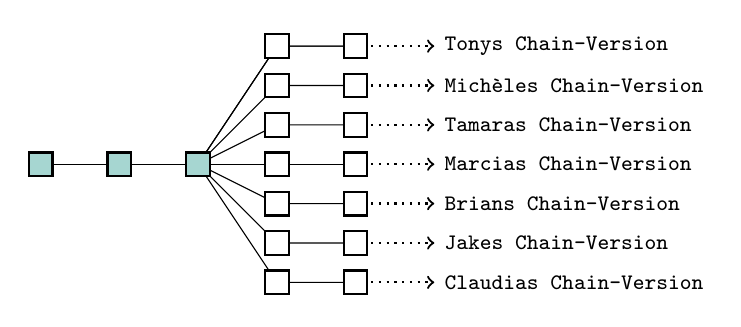
\begin{tikzpicture}[domain=1:10,scale=1, every node/.style={scale=1}]
\coordinate (o1) at (1,1);
\coordinate (o2) at (2,1);
\coordinate (o3) at (3,1);

\coordinate (n1) at (4,2.5);
\coordinate (n2) at (4,2);
\coordinate (n3) at (4,1.5);
\coordinate (n4) at (4,1);
\coordinate (n5) at (4,0.5);
\coordinate (n6) at (4,0);
\coordinate (n7) at (4,-0.5);

\coordinate (n11) at (5,2.5);
\coordinate (n22) at (5,2);
\coordinate (n33) at (5,1.5);
\coordinate (n44) at (5,1);
\coordinate (n55) at (5,0.5);
\coordinate (n66) at (5,0);
\coordinate (n77) at (5,-0.5);

\coordinate (n111) at (6,2.5);
\coordinate (n222) at (6,2);
\coordinate (n333) at (6,1.5);
\coordinate (n444) at (6,1);
\coordinate (n555) at (6,0.5);
\coordinate (n666) at (6,0);
\coordinate (n777) at (6,-0.5);

  \draw[color=black] (o1) to[] (o2) to[] (o3);
  \draw[color=black] (o3) to[] (n1) to[] (n11);
    \draw[color=black] (o3) to[] (n1) to[] (n11);
    \draw[color=black] (o3) to[] (n2) to[] (n22);
    \draw[color=black] (o3) to[] (n3) to[] (n33);
    \draw[color=black] (o3) to[] (n4) to[] (n44);
    \draw[color=black] (o3) to[] (n5) to[] (n55);
    \draw[color=black] (o3) to[] (n6) to[] (n66);
    \draw[color=black] (o3) to[] (n7) to[] (n77);
    
  \draw[color=black,thick, dotted, ->] (n11) to[] (n111) node[right]{\texttt{\footnotesize{Tonys Chain-Version}}};
  \draw[color=black,thick, dotted, ->] (n22) to[] (n222) node[right]{\texttt{\footnotesize{Michèles Chain-Version}}};
  \draw[color=black,thick, dotted, ->] (n33) to[] (n333) node[right]{\texttt{\footnotesize{Tamaras Chain-Version}}};
  \draw[color=black,thick, dotted, ->] (n44) to[] (n444) node[right]{\texttt{\footnotesize{Marcias Chain-Version}}};
  \draw[color=black,thick, dotted, ->] (n55) to[] (n555) node[right]{\texttt{\footnotesize{Brians Chain-Version}}};
  \draw[color=black,thick, dotted, ->] (n66) to[] (n666) node[right]{\texttt{\footnotesize{Jakes Chain-Version}}};
  \draw[color=black,thick, dotted, ->] (n77) to[] (n777) node[right]{\texttt{\footnotesize{Claudias Chain-Version}}};

  \node (rect) at (o1) [fill=highlight,draw,thick,minimum width=0.3cm,minimum height=0.3cm] {};
  \node (rect) at (o2) [fill=highlight,draw,thick,minimum width=0.3cm,minimum height=0.3cm] {};
  \node (rect) at (o3) [fill=highlight,draw,thick,minimum width=0.3cm,minimum height=0.3cm] {};
  \node (rect) at (n1) [fill=white,draw,thick,minimum width=0.3cm,minimum height=0.3cm] {};
  \node (rect) at (n11) [fill=white,draw,thick,minimum width=0.3cm,minimum height=0.3cm] {};
  \node (rect) at (n2) [fill=white,draw,thick,minimum width=0.3cm,minimum height=0.3cm] {};
  \node (rect) at (n22) [fill=white,draw,thick,minimum width=0.3cm,minimum height=0.3cm] {};
  \node (rect) at (n3) [fill=white,draw,thick,minimum width=0.3cm,minimum height=0.3cm] {};
  \node (rect) at (n33) [fill=white,draw,thick,minimum width=0.3cm,minimum height=0.3cm] {};
  \node (rect) at (n4) [fill=white,draw,thick,minimum width=0.3cm,minimum height=0.3cm] {};
  \node (rect) at (n44) [fill=white,draw,thick,minimum width=0.3cm,minimum height=0.3cm] {};
  \node (rect) at (n5) [fill=white,draw,thick,minimum width=0.3cm,minimum height=0.3cm] {};
  \node (rect) at (n55) [fill=white,draw,thick,minimum width=0.3cm,minimum height=0.3cm] {};
  \node (rect) at (n6) [fill=white,draw,thick,minimum width=0.3cm,minimum height=0.3cm] {};
  \node (rect) at (n66) [fill=white,draw,thick,minimum width=0.3cm,minimum height=0.3cm] {};
  \node (rect) at (n7) [fill=white,draw,thick,minimum width=0.3cm,minimum height=0.3cm] {};
  \node (rect) at (n77) [fill=white,draw,thick,minimum width=0.3cm,minimum height=0.3cm] {};
\end{tikzpicture}    
	\end{figure}
\vspace{1em}
Each of these nodes believes that its own block candidate should be added to the blockchain and will ignore those of other network participants.
\end{frame}

%%%

\end{document}